\documentclass[landscape,final,a0paper,fontscale=0.285]{baposter}


\usepackage{calc}
\usepackage{graphicx}
\usepackage{amsmath}
\usepackage{amssymb}
\usepackage{relsize}
\usepackage{multirow}
\usepackage{rotating}
\usepackage{bm}
\usepackage{url}

\usepackage{graphicx}
\usepackage{multicol}

%\usepackage{times}
%\usepackage{helvet}
%\usepackage{bookman}
\usepackage{palatino}

\newcommand{\captionfont}{\footnotesize}

\graphicspath{{images/}{../images/}}
\usetikzlibrary{calc}

%%%%%%%% begin tikz %%%%%%
\usepackage{tikz,tkz-base}
\usetikzlibrary{shapes,decorations,shadows}
\usetikzlibrary{decorations.pathmorphing}
\usetikzlibrary{decorations.shapes}
\usetikzlibrary{fadings}
\usetikzlibrary{patterns}
\usetikzlibrary{calc}
\usetikzlibrary{decorations.text}
\usetikzlibrary{decorations.footprints}
\usetikzlibrary{decorations.fractals}
\usetikzlibrary{shapes.gates.logic.IEC}
\usetikzlibrary{shapes.gates.logic.US}
\usetikzlibrary{fit,chains}
\usetikzlibrary{positioning}
\usepgflibrary{shapes}
\usetikzlibrary{scopes}
\usetikzlibrary{arrows}
\usetikzlibrary{backgrounds}


\tikzset{latent/.style={circle,fill=white,draw=black,inner sep=1pt, 
minimum size=20pt, font=\fontsize{10}{10}\selectfont},
obs/.style={latent,fill=gray!25},
const/.style={rectangle, inner sep=0pt},
factor/.style={rectangle, fill=black,minimum size=5pt, inner sep=0pt},
>={triangle 45}}


\pgfdeclarelayer{b}
\pgfdeclarelayer{f}
\pgfsetlayers{b,main,f}

% shapename, fitlist, caption, pos
\newcommand{\plate}[4]{
\begin{pgfonlayer}{b}
\node (invis#1) [draw, color=white, inner sep=1pt,rectangle,fit=#2] {};
\end{pgfonlayer}\begin{pgfonlayer}{f}
\node (capt#1) [ below left=0 pt of invis#1.south east, xshift=2pt,yshift=1pt] {\footnotesize{#3}};
\node (#1) [draw,inner sep=1pt, rectangle,fit=(invis#1) (capt#1),#4] {};
\end{pgfonlayer}
}


\newcommand{\shiftedplate}[5]{
\begin{pgfonlayer}{b}
\node (invis#1) [draw, color=white, inner sep=0 pt,rectangle,fit=#2] {};
\end{pgfonlayer}\begin{pgfonlayer}{f}
\node (capt#1) [#5, xshift=2pt] {\footnotesize{#3}};
\node (#1) [draw,inner sep=2pt, rectangle,fit=(invis#1) (capt#1),#4] {};
\end{pgfonlayer}
}

%shapename, pos, caption, in1, in2, out, captpos
\newcommand{\twofactor}[7]{
\node (#1) [factor] at #2 {};
\node (capt#1) [#7 of #1]{\footnotesize{#3}};
\draw [-] (#4) -- (#1) ;
\draw [-] (#5) -- (#1) ;
\draw [->,thick] (#1) -- (#6);
}

%shapename, pos, caption, in, out, captpos
\newcommand{\factor}[6]{
\node (#1) [factor] at #2 {};
\node (capt#1) [#6 of #1]{\footnotesize{#3}};
\draw [-] (#4) -- (#1) ;
\draw [->,thick] (#1) -- (#5);
}

% name, --, caption, pos
\newcommand{\nofactor}[4]{
\node (#1) [factor, #2]  {};
\node (capt#1) [#4 of #1]{\footnotesize{#3}};
}

%shapename,  fitlist, caption
\newcommand{\namedgate}[3]{
\begin{pgfonlayer}{b}
\node (invisgate#1) [rectangle, draw, color=white,  fit=#2] {};
\end{pgfonlayer}
\node (gatecapt#1) [ above right=0 pt of invisgate#1.north west, xshift=-1pt ] {\footnotesize{#3}};
\node (#1) [rectangle,draw,dashed, inner sep=2pt, fit=(invisgate#1)(gatecapt#1)]{};

}

%shapename,  fitlist, caption
\newcommand{\gate}[3]{
\node (#1) [rectangle,draw,dashed, inner sep=2pt, fit=#2]{};
}

%shapename,  fitlist1, fitlist2, caption1, caption2
\newcommand{\vertgate}[5]{
\begin{pgfonlayer}{b}
\node (invisgateleft#1) [rectangle, draw, color=white,  fit=#2] {};
\node (invisgateright#1) [rectangle, draw, color=white,  fit=#4] {};
\end{pgfonlayer}
\node (gatecaptleft#1) [ above left=0 pt of invisgateleft#1.north east, xshift=1pt ]{\footnotesize{#3}};
\node (gatecaptright#1) [ above right=0 pt of invisgateright#1.north west, xshift=-1pt ] {\footnotesize{#5}};
\node (#1) [rectangle,draw,dashed, inner sep=2pt, fit=(invisgateleft#1)(gatecaptleft#1)(invisgateright#1)(gatecaptright#1)]{};
\draw [-, dashed] (#1.north) -- (#1.south);
}


\newcommand{\vertgateSpec}[5]{
\begin{pgfonlayer}{b}
\node (invisgateleft#1) [rectangle, draw, color=white,  fit=#2] {};
\node (invisgateright#1) [rectangle, draw, color=white,  fit=#4] {};
\end{pgfonlayer}
\node (gatecaptleft#1) [ above left=0 pt of invisgateleft#1.north east, xshift=1pt ]{\footnotesize{#3}};
\node (gatecaptright#1) [ above right=0 pt of invisgateright#1.north west, xshift=-1pt ] {\footnotesize{#5}};
\node (#1) [rectangle,draw,dashed, inner sep=2pt, fit=(invisgateleft#1)(gatecaptleft#1)(invisgateright#1)(gatecaptright#1)]{};
\draw [-, dashed] (#1.70) -- (#1.290);
}

\newcommand{\horgate}[5]{
\begin{pgfonlayer}{b}
\node (invisgateleft#1) [rectangle, draw, color=white,  fit=#2] {};
\node (invisgateright#1) [rectangle, draw, color=white,  fit=#4] {};
\end{pgfonlayer}
\node (gatecaptleft#1) [ above right=0 pt of invisgateleft#1.south west, xshift=1pt ]{\footnotesize{#3}};
\node (gatecaptright#1) [ below right=0 pt of invisgateright#1.north west, xshift=-1pt ] {\footnotesize{#5}};
\node (#1) [rectangle,draw,dashed, inner sep=2pt, fit=(invisgateleft#1)(gatecaptleft#1)(invisgateright#1)(gatecaptright#1)]{};
\draw [-, dashed] (#1.west) -- (#1.east);
}

\newcommand{\horogate}[5]{
\begin{pgfonlayer}{b}
\node (invisgateleft#1) [rectangle, draw, color=white,  fit=#2] {};
\node (invisgateright#1) [rectangle, draw, color=white,  fit=#4] {};
\end{pgfonlayer}
\node (#1) [rectangle,draw,dashed, inner sep=2pt, fit=(invisgateleft#1)(invisgateright#1)]{};
\node (gatecaptleft#1) [ above right=0 pt of #1.west, xshift=0pt ]{\footnotesize{#3}};
\node (gatecaptright#1) [ below right=0 pt of #1.west, xshift=0pt ] {\footnotesize{#5}};

\draw [-, dashed] (#1.west) -- (#1.east);
}


\newcommand{\vertogate}[5]{
\begin{pgfonlayer}{b}
\node (invisgateleft#1) [rectangle, draw, color=white,  fit=#2] {};
\node (invisgateright#1) [rectangle, draw, color=white,  fit=#4] {};
\end{pgfonlayer}
\node (#1) [rectangle,draw,dashed, inner sep=2pt, fit=(invisgateleft#1)(invisgateright#1)]{};
\node (gatecaptleft#1) [ below left=0 pt of #1.north, xshift=0pt ]{\footnotesize{#3}};
\node (gatecaptright#1) [ below right=0 pt of #1.north, xshift=0pt ] {\footnotesize{#5}};

\draw [-, dashed] (#1.north) -- (#1.south);
}



\newcommand{\SET}[1]  {\ensuremath{\mathcal{#1}}}
\newcommand{\MAT}[1]  {\ensuremath{\boldsymbol{#1}}}
\newcommand{\VEC}[1]  {\ensuremath{\boldsymbol{#1}}}
\newcommand{\Video}{\SET{V}}
\newcommand{\video}{\VEC{f}}
\newcommand{\track}{x}
\newcommand{\Track}{\SET T}
\newcommand{\LMs}{\SET L}
\newcommand{\lm}{l}
\newcommand{\PosE}{\SET P}
\newcommand{\posE}{\VEC p}
\newcommand{\negE}{\VEC n}
\newcommand{\NegE}{\SET N}
\newcommand{\Occluded}{\SET O}
\newcommand{\occluded}{o}

\begin{document}
  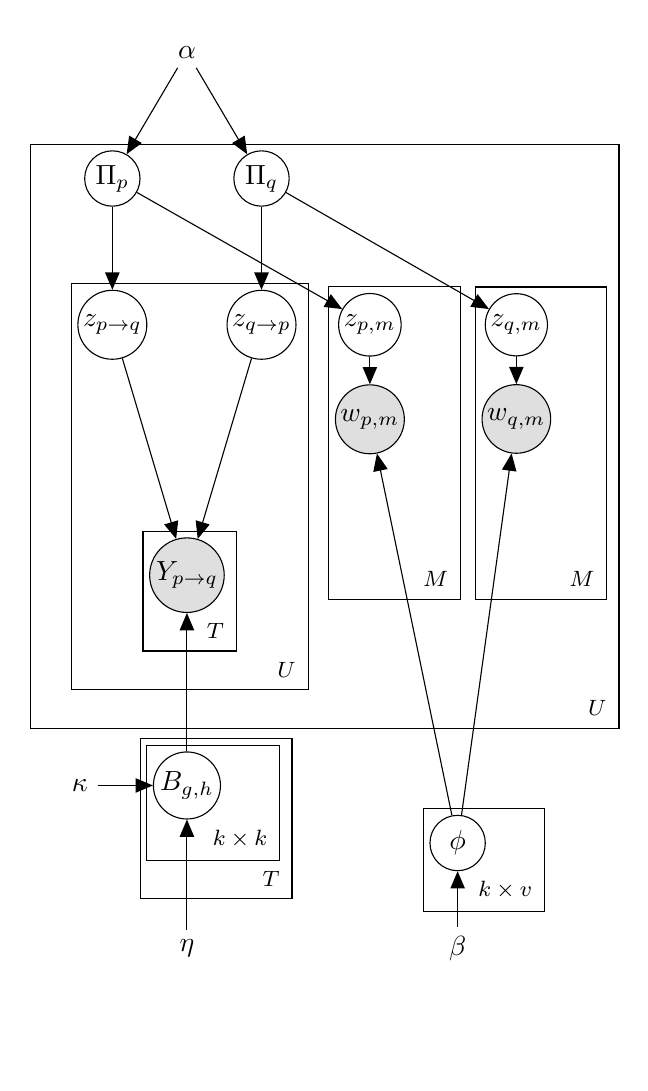
\begin{tikzpicture}
    \node [matrix,matrix anchor=mid, column sep=10pt, row sep=30pt] {

    \node (alpha) {$\alpha$};
    \\

    \node (pi_p) [latent, left = 10pt of alpha] {$\Pi_{p}$};
    \node (pi_q) [latent, right = 10pt of alpha] {$\Pi_{q}$};

    \\
    \node (z_pq) [latent, above = 15pt of pi_p] {$z_{p \rightarrow q}$};
    \node (z_qp) [latent, above = 15pt of pi_q] {$z_{q \rightarrow p}$};

    \node (z_um) [latent, right = 15pt of z_qp] {$z_{p,m}$};

    \node (w_um) [obs, below = 10pt of z_um] {$w_{p,m}$};

    \node (z_um2) [latent, right = 30pt of z_um] {$z_{q,m}$};

    \node (w_um2) [obs, below = 10pt of z_um2] {$w_{q,m}$};


    \\
    \node (Y_pq) [obs, above = 10pt of alpha] {$Y_{p \rightarrow q}$};

    \node (spaceleft) [rectangle, draw, transparent,  left = 10pt of pi_p] {};
    \node (spaceright) [rectangle, draw, transparent,  right = 10pt of pi_q] {};
    \node (spaceabove) [rectangle, draw, transparent, above = 10pt of pi_p] {};
    \node (plate1_plat2_spc) [rectangle, draw, transparent, left = 10pt of z_qp] {};

    \node (b_gh) [latent, below = 50pt of Y_pq] {$B_{g,h}$};

    \node (spaceleft_block_plate) [rectangle, draw, transparent, right = 10pt of b_gh] {};


    \node (eta) [below = 40pt of b_gh] {$\eta$};

    \node (beta) [below = 150pt of alpha, right = 85pt of eta] {$\beta$};

    \node [latent, above = 20pt of beta] (tau) {$\phi$};

    \node (spaceleft_tau_plate) [rectangle, draw, transparent, right = 10pt of tau] {};

    \node (spaceleft_pi2zum_plate) [rectangle, draw, transparent, right = 10pt of z_um] {};

    \node (spaceleft_pi2zum2_plate) [rectangle, draw, transparent, right = 10pt of z_um2] {};

    \node (kappa) [left = 20pt of b_gh] {$\kappa$}; 
    \\
    \\
    };
    \plate{y_plate}{(Y_pq)}{$T$}{}
    \plate{pi_p_to_z}{(z_pq)(z_qp)(y_plate)}{$U$}{};
    \plate{pi_p_to_z_um}{(spaceleft_pi2zum_plate)(z_um)(w_um)}{$M$}{};
    \plate{pi_p_to_z_um2}{(spaceleft_pi2zum2_plate)(z_um2)(w_um2)}{$M$}{};
    \plate{p}{(pi_p_to_z)(plate1_plat2_spc)(pi_p_to_z_um)(pi_p_to_z_um2)(spaceleft)(spaceright)(spaceabove)(pi_p)(pi_q)}{$U$}{};

    \plate{blockplate}{(spaceleft_block_plate)(b_gh)}{$k \times k$}{};
    \plate{t_plate}{(blockplate)}{$T$}{};

    \plate{tauplate}{(spaceleft_tau_plate)(tau)}{$k \times v$}{};

    \draw [->] (alpha) -- (pi_p);
    \draw [->] (alpha) -- (pi_q);

    \draw [->] (pi_p) -- (z_pq);
    \draw [->] (pi_q) -- (z_qp);

    \draw [->] (pi_p) -- (z_um);
    \draw [->] (pi_q) -- (z_um2);
    \draw [->] (z_um) -- (w_um);
    \draw [->] (z_um2) -- (w_um2);

    \draw [->] (z_pq) -- (Y_pq);
    \draw [->] (z_qp) -- (Y_pq);

    \draw [->] (b_gh) -- (Y_pq);
    \draw [->] (eta) -- (b_gh);

    \draw [->] (beta) -- (tau);
    \draw [->] (tau) -- (w_um);
    \draw [->] (tau) -- (w_um2);

    \draw [->] (kappa) -- (b_gh);

  \end{tikzpicture}
  \end{document}
